\chapter{Workflow and Customer Journey for Coffee Chain ERP System}

This chapter details how administrators configure the system and how customers experience transactions at outlets. The workflows highlight the sequence of operations, responsibilities, and ERP automation. Presenting the workflow from multiple perspectives helps readers understand how each actor interacts with the ERP system and how data flows throughout the organization.

\section*{System Entities}
The ERP system manages multiple entities critical for operations. Table~\ref{tab:entities} summarizes the primary entities.

\begin{table}[H]
\centering
\begin{tabular}{|l|p{10cm}|}
\hline
\textbf{Entity} & \textbf{Description} \\ \hline
\texttt{coffee.outlet} & Coffee Outlet details, including location, operational hours, and assigned managers. \\ \hline
\texttt{res.partner} & Represents both outlet owners and sale customers, enabling traceable transactions and CRM integration. \\ \hline
\texttt{coffee.menu.item} & Menu Items with categories (drinks, snacks, combos) and pricing. \\ \hline
\texttt{sale.order} & Captures customer orders linked to specific outlets and menu items. \\ \hline
\texttt{crm.lead} & Optional CRM Leads used for marketing and customer engagement tracking. \\ \hline
\end{tabular}
\caption{Primary System Entities}
\label{tab:entities}
\end{table}

\section*{Administrator Workflow}
Administrators configure the backbone of the ERP system. Proper setup ensures consistent operations across outlets and accurate reporting. The typical workflow includes:

\begin{enumerate}
    \item Create outlet profiles, assign managers, and set operational details such as working hours and location coordinates.  
    \item Populate the Menu Master with drinks, snacks, combos, and their corresponding pricing.  
    \item Register sale customers in the system for traceable transactions.  
    \item Optionally link CRM leads for customer engagement tracking and marketing campaigns.  
\end{enumerate}

\begin{figure}[H]
    \centering
    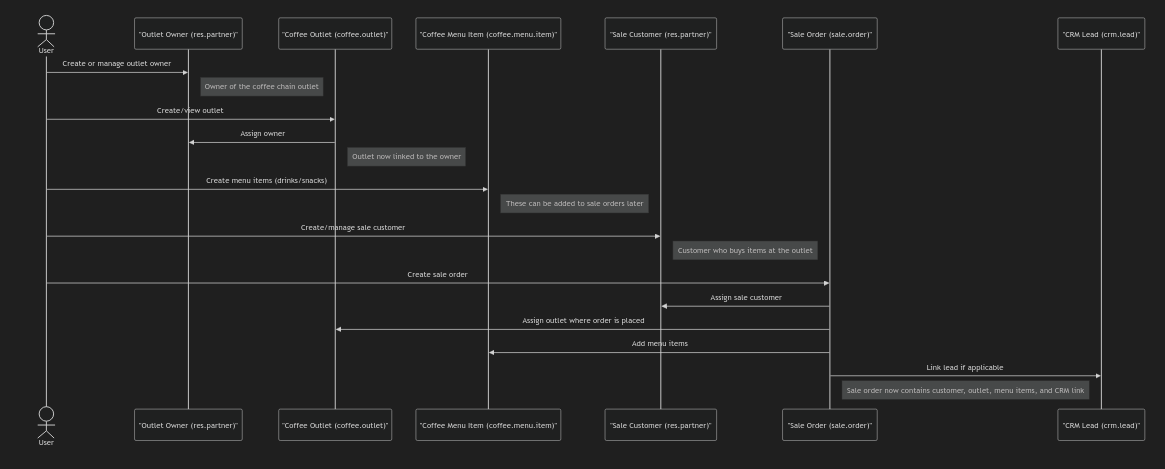
\includegraphics[width=0.85\textwidth]{diagrams/sequence.png}
    \caption{Administrator Workflow Sequence Diagram. Proper configuration ensures smooth operations across outlets.}
    \label{fig:admin_workflow}
\end{figure}

\begin{tcolorbox}[colback=white,colframe=odooPurple,title=Tip, fonttitle=\bfseries, coltitle=white]
Ensure all outlets have assigned managers and accurate operational hours to avoid discrepancies in daily reporting.
\end{tcolorbox}

\section*{Customer Journey Through Perspectives}
The ERP system streamlines interactions for all stakeholders. Explaining the customer journey through multiple perspectives illustrates the practical impact of the system.

\subsection*{1. Customer's Point of View}
\textit{Scenario: Anna visits a coffee outlet on a busy morning.}

\begin{enumerate}
    \item Anna browses the menu displayed at the counter or digital screen.  
    \item She selects a cappuccino and a croissant.  
    \item Places her order with the staff and completes payment.  
    \item Receives a receipt instantly and waits for the order.  
\end{enumerate}

\begin{tcolorbox}[colback=white,colframe=odooPurple,title=Tip, fonttitle=\bfseries, coltitle=white]
If the customer is registered, loyalty points are updated automatically, improving engagement and repeat business.
\end{tcolorbox}

From the customer's perspective, the experience is seamless, fast, and accurate because the ERP automates order capture and billing.

\subsection*{2. Barista / Staff Point of View}
\textit{Scenario: The staff prepares Anna's order and manages the transaction.}

\begin{enumerate}
    \item Selects the outlet profile in the ERP system to ensure orders are linked correctly.  
    \item Adds Anna’s menu items to a new sale order in the system.  
    \item Confirms the order, processes payment, and prints the receipt.  
    \item ERP automatically updates inventory levels and notifies the preparation team.  
    \item Marks the order ready for delivery or pickup, maintaining workflow efficiency.  
\end{enumerate}

\begin{tcolorbox}[colback=white,colframe=odooPurple,title=Note, fonttitle=\bfseries, coltitle=white]
Inventory levels are updated in real-time, helping staff avoid overselling items that are out of stock.
\end{tcolorbox}

\subsection*{3. Manager's Point of View}
\textit{Scenario: The outlet manager monitors daily operations and sales.}

\begin{enumerate}
    \item Reviews incoming orders and overall sales in real-time dashboards.  
    \item Monitors staff efficiency and customer service metrics.  
    \item Tracks product demand and inventory levels for restocking and promotions.  
    \item Uses CRM data to plan marketing campaigns or customer engagement initiatives.  
    \item Analyzes reports generated automatically by the ERP for operational and strategic decision-making.  
\end{enumerate}

\begin{figure}[H]
    \centering
    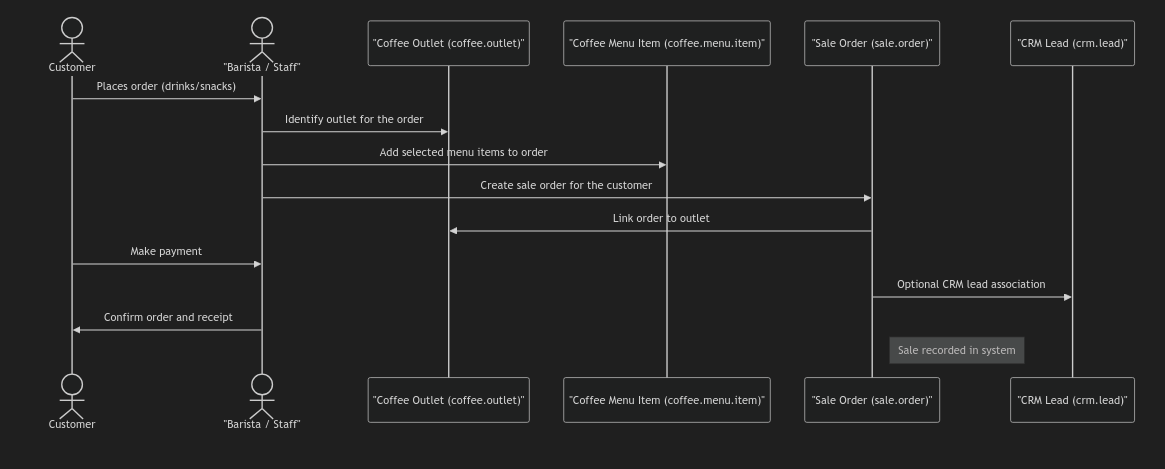
\includegraphics[width=0.85\textwidth]{diagrams/customer_journey.png}
    \caption{Customer Journey Sequence Diagram showing interactions from customer, staff, and manager perspectives.}
    \label{fig:customer_journey}
\end{figure}

\section*{Insights}
\begin{itemize}
    \item Administrators create the foundation; customers generate daily operational data.  
    \item ERP workflows ensure traceability of every transaction and maintain data integrity.  
    \item The system links customer experiences directly with business reporting, enabling informed decisions.  
\end{itemize}
